The simulated data after the detector simulation described in \Sec{sec:eventgeneration}, has the exact same format as the real collision data recorded by the CMS experiment. Therefore the same software can be used for the reconstruction of both simulation and real data. In \Sec{sec:reco}, the object reconstruction is explained. After reconstructing the objects, they are connected to physics objects, which need to be identified (\Sec{sec:PF}) and corrected for pileup (\Sec{sec:pileup}). The objects used for physics analysis have extra requirements as shown in \Sec{sec:PhysicsObject}. A summary of all the corrections applied to data and simulation is given in \Sec{sec:SummaryCor}.

\section{Object Reconstruction}
\label{sec:reco}
In \fig{fig:transversecms}, the particle interaction in a transverse slice of the CMS detector is shown. When a particle is created in the collisions in the detector, it first enters the tracker where charged particle trajectories, so-called tracks, and origins, so-called vertices, are reconstructed from signals or hits in the sensitive layers. The  magnetic field bends the charged particles making it able to measure the electric charges and momenta of charged particles. The electrons and photons are absorbed in the ECAL and the corresponding electromagnetic showers are detected as clusters of energy in adjacent cells. From this, the energy and the direction of the particles can be determined. The charged and neutral hadrons initiate a hadronic shower in the ECAL, and their showers are fully absorbed in the HCAL. The clusters from these showers are used to estimate the energy and direction of the hadrons. Muons and neutrinos pass through the calorimeters without little to no energy loss and the neutrinos even escape the CMS detector undetected while muons produce hits in the muon detectors. 
\begin{landscape}
\begin{figure}
	\centering
	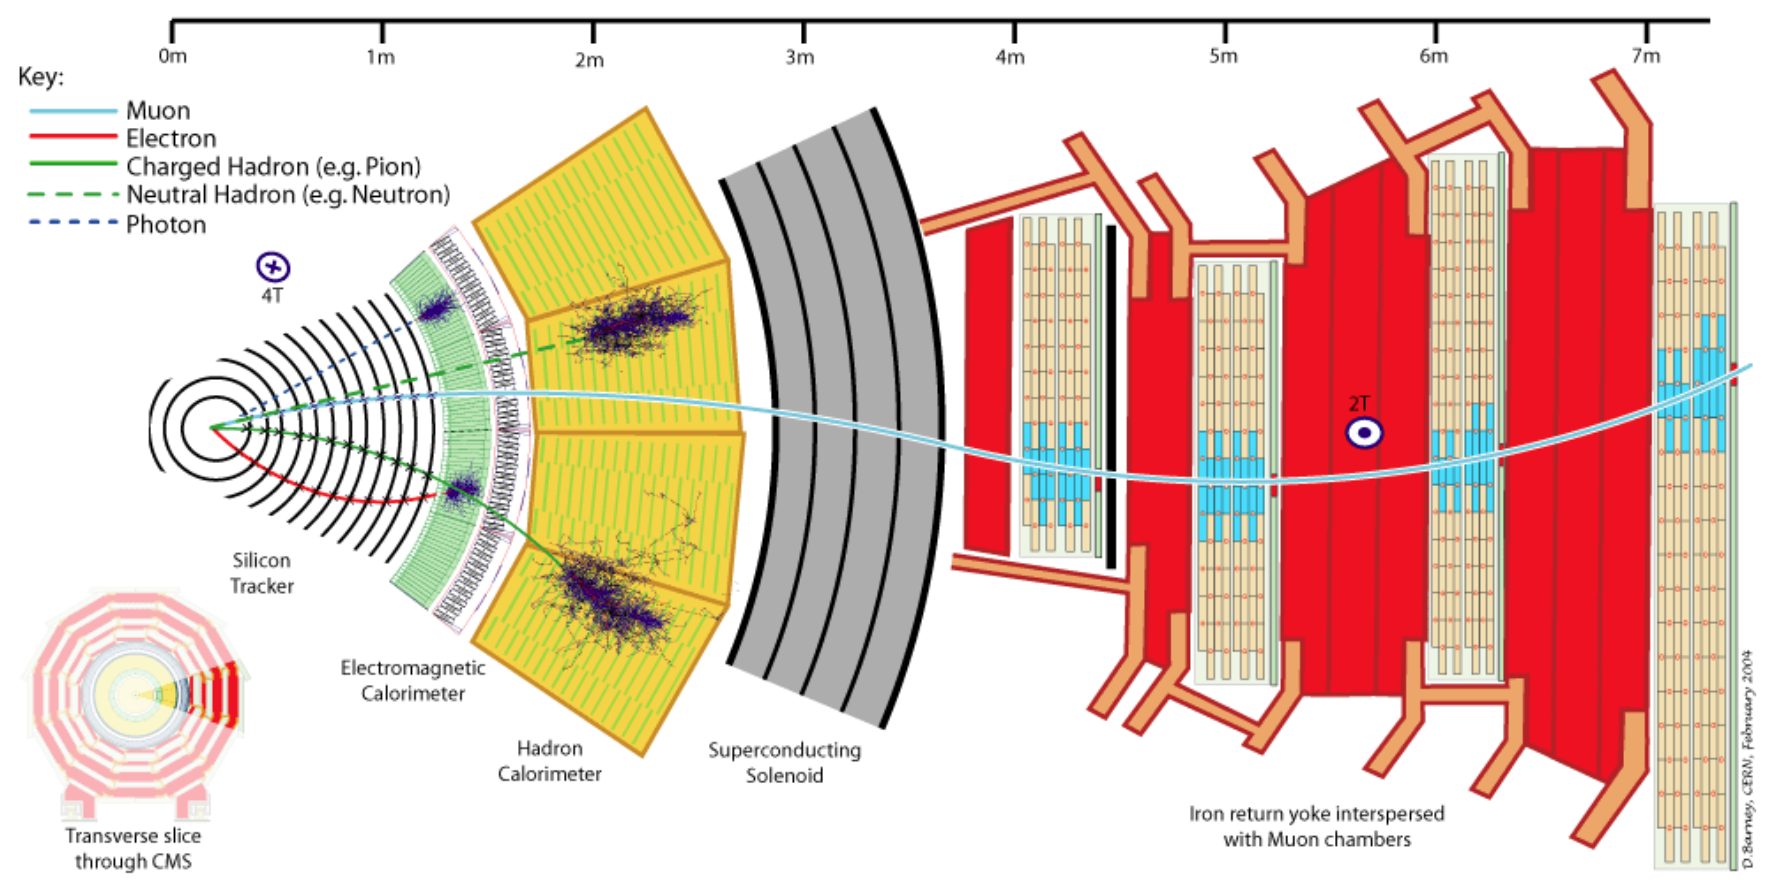
\includegraphics[width=1.\linewidth]{4_EventRecoSelect/Figures/transversecms}
	\caption{Cross-section of the CMS detector with all parts of the detector labelled. This sketch shows the specific particle interactions from a beam interaction reaching the muon detector. The muon and charged pion are positively charged, the electron is negatively charged. Figure taken from~\cite{CMS-PRF-14-001}. }
	\label{fig:transversecms}
\end{figure}
\end{landscape}
%The traditional hadron colliders reconstruction is as follows. The reconstruction of isolated photons and electrons is primarily done by the ECAL, while the identification of muons is based on the muon detectors. Hadrons and photons form jets which are measured by the calorimeters without any contribution from the tracker or muon detectors. Jets can be tagged using the tracker as coming from hadronic \Ptau\ decays or \Pbottom\ hadronisation based on the properties of the relevant charged particle tracks. The missing transverse energy \ptmisvec\ is defined as the vectorial sum of the undetectable particle transverse momenta, and can be reconstructed without any information from the tracker. 
The particle flow (PF)~\cite{CMS-PRF-14-001} reconstruction algorithm correlates the tracks and clusters from all detector layers with the identification of each final state particle, and combines the corresponding measurements to reconstruct their properties. The muon is identified by a track in the inner tracker, connected to a track in the muon detector as described in \Sec{sec:MuonTrack}. The electrons are identified by a track and an ECAL cluster, not connected to an HCAL cluster as described in \Sec{sec:ElectronTrack}. The ECAL and HCAL clusters without a track link identify the photons and neutral hadrons, while the addition of the tracker determines the energy and direction of a charged hadron (\Sec{sec:calo}). 


%Coarse-grained detectors can cause signals of different particles to merge and reduce the ability of identifying and reconstructing the particles. Therefore, particle flow identification requires sufficiently segmented subdetectors such that a global event description is possible. The CMS detector is built to meet to requirements of the particle flow reconstruction. It has an efficient and pure muon identification system, a hermetic HCAL with coarse segmentation, a higher segmented ECAL, a fine-grained tracker and a large magnetic field to separate the calorimeter deposits of charged and neutral particles in jets. 

%http://slideplayer.com/slide/2779564/
%http://slideplayer.com/slide/4496166/
\subsection{Charged particle tracks}
An iterative tracking algorithm is responsible for the reconstruction of the tracks made by charged particles in the inner tracking system. Each iteration consists of four steps~\cite{Bayatian:922757}: the track-seed generation, the pattern recognition algorithm, removal of track-hit ambiguities and a final track fit. The pattern recognitions are done by use the Kalman filter method~\cite{FRUHWIRTH1987444,Billoir:1989mh} which takes into account the magnetic field and multiple scattering effects. All hits that are unambiguously associated to the final track are removed from the list of available hits. In order to associate the remaining hits, the procedure is repeated with looser track reconstruction criteria. The use of the iterative track reconstruction procedure has a high track finding efficiency, where the fake track reconstruction rate is negligible. 
%For muons, this results in a global track reconstruction efficiency exceeding 98\%, and 75-98\% for charged hadrons. 

\subsection{Following the Muon's Footsteps}
\label{sec:MuonTrack}
% see http://www.bo.infn.it/sminiato/sm16/03_Mercoledi/Mattina/01_Battilana.pdf
% see https://arxiv.org/pdf/1510.05424.pdf
% see https://twiki.cern.ch/twiki/bin/view/CMSPublic/MuonDPGPublic160729
The muon reconstruction~\cite{Chatrchyan:2012xi} has three subdivisions: local reconstruction, regional reconstruction and global reconstruction. The local reconstruction is performed on individual detector elements such as strip and pixel hits in the inner tracking system, and muon hits and/or segments in the muon chambers. Independent tracks are reconstructed in the inner tracker, so-called tracker tracks, and in the muon system, so-called standalone muon tracks. Based on these tracks, two reconstructions are considered: Global Muon reconstruction and Tracker Muon reconstruction. The first one is an outside-in approach starting from a standalone muon track while the second one uses an inside-out approach starting from tracker tracks. For low transverse momenta ($\pt \lesssim$ 5~\GeV), the tracker muon reconstruction is  more efficient than the global muon approach. This is due to the fact that tracker muons only require a single muon  segment in muon system, while the global muon approach requires typically segments in at least two muon stations. These tracker muons are used for identifying muons from the hadronisation of \Pbottom\ or \Pcharm\  quarks. The global muon approach typically improves the tracker reconstruction for $\pt\gtrsim$ 200~\GeV. %These are labelled isolated when in a cone of $\Delta R = \sqrt{\Delta\phi^2 + \Delta \eta^2} = 0.3$ around the muon, the sum of the transverse momenta of additional tracker tracks and energy deposits in the calorimeter is less than 10\% of the muon's transverse momentum.

%The outside-in approach is referred to as Global Muon reconstruction. 
%For each standalone muon track, a inner tracker track is found by comparing the parameters of the two tracks propagated onto a common surface. Combining the hits from the tracker track and the standalone track, gives a fit via the Kalman filter technique~\cite{FRUHWIRTH1987444,Billoir:1989mh} for a global muon track. 
%
%The second approach is an inside-out reconstruction, creating tracker muons. 
%All candidate tracker tracks with a \pt$>0.5$ \GeV\ and total momentum p$>2.5$ \GeV\ are extrapolated to the muon system taking into account the magnetic field, the average expected energy losses, and multiple Coulomb scattering in the detector material. The extrapolated track and the muon segments are considered matched when the difference in the position in the x coordinates is smaller than 3~\cm, or when the ratio of this distance to its uncertainty is smaller than four. When at least one muon segment - DT or CSC hits -  matches the extrapolated track, the corresponding tracker track is indicated as a tracker muon. 


\subsection{The path of the Electron}
\label{sec:ElectronTrack}
% see also https://arxiv.org/pdf/physics/0512097.pdf
% https://cds.cern.ch/record/1563583/files/ATL-PHYS-PROC-2013-206.pdf
% http://cds.cern.ch/record/1704291
 Standard tracking algorithms are based on Kalman filtering which assume that the energy loss is Gaussian distributed. Since the  electron tracks are increasingly curved in the magnetic field as a function of its flight distance, these standard tracking algorithms are not suitable to fit the electron tracks. The Gaussian sum filter (GSF)~\cite{0954-3899-31-9-N01} is used instead. 

In CMS, the electrons are reconstructed in two ways. The older ECAL based tracking is developed to identify high energetic isolated electrons. This tracking algorithm starts from ECAL clusters with a transverse energy above 4~\GeV\ and extrapolates from these cluster the position of the hits in the tracker. Another, tracker based algorithm uses all the tracks with a \pt\ higher than 2~\GeV\ found with iterative tracking as seeds. The electron seeds from the ECAL- and tracker-based procedures are merged into a unique collection and are then refitted  by using the summed Gaussian distributions as uncertainty per hit in the track fit. The electron efficiency is measured in 8~\TeV\ proton collision data to be better than 93\% for electrons with an ECAL supercluster energy of $E_{\mathrm{T}}>20$~\GeV~\cite{1748-0221-10-06-P06005}. For electrons with an  $E_{\mathrm{T}}>25$~\GeV\  in 13~\TeV\ proton collision data, the efficiency is about 96\%~\cite{CMS-DP-2017-004}.


%This tracker algorthm has two main downsides that it is prone to extrapolating a wring position in the tracker and will miss energy deposits
%
%
%In order to account for bremsstrahlung, neighbouring clusters in $\eta$ and $\phi$
%are grouped together into a supercluster from which then the direction is determined to find the position of the particles in the tracker. This has as consequence that for electrons or positrons in jets, energy deposits of surrounding particles will be entering the supercluster leading to a wrong position of the electron/positron in the tracker. Another disadvantage of the ECAL based tracking is that for low \pt\ electrons, the trajectories will be very curved and the supercluster will not contain all of the energy deposit, leading to a higher misconstruction rate. 
%
%The faults of the ECAL based tracking are lifted by adding a tracker based algorithm. This algorithm uses all the tracks with a \pt\ higher than 2~\GeV\ found with iterative tracking as seeds. Iterative tracking uses the Kalman Filter algorithm several times with an average track reconstruction efficiency but high purity. In contrary with a global combinatorial fit, the iterative tracking accepts tracks with a small transverse momentum that are not leaving any energy in the ECAL, and tracks from particles that only interact with the inner tracker layers. When the electron or positron radiated a small amount of energy, the corresponding track can be reconstructed across the whole tracker and safely propagated to the ECAL surface. When there is a larger amount of energy radiated however, the pattern recognition might fail  to accommodate for the change in the electron momentum leading to a track reconstructed with a small number of hits. The solution for this is a preselection based on the $\chi^2$ and number of hits and the selected tracks are fitted again with Gaussian-Sum-Filter which can accommodate substantial energy losses across the trajectory. 



%Due to the lack of coverage of the two pixel discs in high \abspsrap range, the efficiency drops. 
%The resolution on the transverse momentum for a 100 \si{ \GeV} charged particle is about 2.0\% (FIX ME). 
% see https://twiki.cern.ch/twiki/bin/view/CMSPublic/TrackingPOGPlots2016
\subsection{Primary Vertex Reconstruction}
The primary vertex (PV) reconstruction is able to measure the location of all proton interaction vertices in each event consisting of the signal vertex and all vertices from pileup events. First, tracks are selected  to be consistent with being produced promptly in the primary interaction~\cite{Chatrchyan:1704291}. Then the tracks are grouped according to the $z$ coordinate of their closest approach to the beam line~\cite{726788} and a vertex fitting algorithm~\cite{Waltenberger:1166320} is performed. The primary vertex is found as the vertex corresponding to the highest sum of squared track transverse momenta and is taken to be the main interaction point. The resolution on the primary vertex is about 14 \si{ \micro \meter} in $r\phi$ and about 19 \si{ \micro \meter} in the $z$ direction for primary vertices with the sum of the track $p_T > 100$ \si{ \GeV} for the 2016 data taking period. A primary vertex is considered a well reconstructed primary vertex when it has at least five degrees of freedom, the longitudinal distance from the beam spot is maximally 24~cm ($d_z < 24$~cm), and the transversal distance from the beam spot is maximally 2~cm ($d_{xy}<2$~cm). 
% numbers from https://twiki.cern.ch/twiki/bin/view/CMSPublic/TrackingPOGPlotsICHEP2016

\subsection{Calorimeter clusters}
\label{sec:calo}
The energy and direction of stable neutral particles such as photons and neutral hadrons are reconstructed using a cluster algorithm.  This algorithm also separates neutral particles from charged hadron energy deposits, 
and reconstructs and identifies electrons and their bremsstrahlung photons. Furthermore, the cluster algorithm is contributing to the energy measurements of charged hadrons that don't have accurate track parameters, e.g. for low quality tracks and high transverse momentum tracks. The clustering is performed separately in each subdetetector: ECAL barrel and endcaps, HCAL barrel and endcaps, and the two preshower layers. The HF has no clustering algorithm since the electromagnetic or hadronic components give rise to an HF EM or HF HAD cluster. 

The clustering algorithm consist of different steps. First seeds are identified when cells have an energy larger than the seeding threshold and larger than their neighbouring cells. Then topological clusters are made by accumulating cells that share at least a corner with a cell already in the cluster and an energy above a cell threshold set to twice the noise level. The third step is an expectation maximization algorithm that reconstructs the cluster~\cite{CMS-PRF-14-001} and assumes that  the energy deposits are Gaussian distributed. The calorimeter clusters are used for reconstructing photons and neutral hadrons. The  clusters that are not in the vicinity of the extrapolated charged tracks are identified as neutral hadrons or photons. If the energy deposits are in vicinity of charged tracks, such is the case for charged hadrons, the neutral particle energy deposit is measured as an excess over the charged particle deposit. %For this reason, a good calibration of the electromagnetic and hadronic calorimeter is  vital. 

%The ECAL calibration is performed before the hadron cluster calibration or particle identification. For run 1, the ECAL response to electrons and photons as well as the cell-to-cell relative calibration is determined with test beam data, radio active sources, and cosmic ray measurements. For run 2, the collision data collected at 7 and 8~\TeV\ was used to refine the calibration. The effect of the thresholds in the clustering algorithm are estimated from simulated single photons with energies varying from 0.25 to 100~\GeV. The photons used for the calibration should not have a conversion prior to their entrance to ensure the calibration of single clusters. In all ECAL regions and for all energies, the calibrated photon energies agree with the true photon energies within 1\%.
%
%In contrary to the photons, the hadrons deposit in general energy in both ECAL and HCAL. Since the calorimeter response in the HCAL depends on the fraction of shower energy deposited in the ECAL, the ECAL and HCAL cluster energies are recalibrated together to get an estimate of the true hadron energy. Since the calibration is done for hadrons, single neutral hadrons such as $K_{\mathrm{L}}^0$ are used for determining the calibration constants. The hadrons interaction with the tracker material are rejected for the calibration purposes. This calibration is checked with isolated charged hadron selected from early data recorded at $\sqrt{s}=0.9, 2.2$ and 7 \TeV.  

%\section{Putting the pieces together}


%The link between a central tracker track and a calorimeter clusters is made by extrapolating the tracker track to the two layers of the preshower, the ECAL, and the HCAL. If this extrapolated position is within the cluster area, the two are linked. When there are several ECAL or HCAL clusters for the same track, the link with the smallest distance is kept. A dedicated cluster algorithm accounts for the energy of the photons emitted through bremsstrahlung at for photons that have converted to an electron-positron pair. \\The ECAL to HCAL cluster and ECAL to preshower cluster links are established when the cluster position in the more granular calorimeter, ECAL or preshower, is in accordance with the cluster envelope of the less granular calorimeter, HCAL or ECAL.  When there are multiple HCAL clusters linked to the same ECAL cluster, the link with the smallest distance is kept. This is also true for multiple ECAL clusters with the same preshower clusters. The ECAL supercluster is linked with the ECAL cluster when they share at least one ECAL cell. \\
%Nuclear interactions in the tracker can lead to kinks in hadron trajectories as well as the production of secondary particles. This leads to charged particle tracks linked together via a common displaced vertex. The displaced vertices considered should have at least three tracks, with at most one incoming track, and the invariant mass of the outgoing tracks should exceed 0.2~\GeV. \\
%The link between a track and the muon detectors is done via local, regional, and global reconstruction as explained in \Sec{sec:MuonTrack}. 


\section{Particle flow identification}
\label{sec:PF}
The several PF elements from the various CMS subdetectors are connected through a link algorithm. This algorithm tests nearest neighbour pairs of elements in an event. The quality of the link is determined via the distance between the two elements and PF blocks of elements are formed from elements with a direct link or indirect link through common elements. The identification and reconstruction follows a particular order in each PF block. After each identification and reconstruction the corresponding PF elements (tracks and clusters) are removed from the PF block.

 The muons are the first to be identified and reconstructed. These are reconstructed if their momenta are compatible with corresponding track only momenta. Then the electrons and their corresponding brehmstrahung photons, are identified and reconstructed by using the GSF tracking. At the same time, the energetic and isolated photons are identified as well. The remaining elements in the PF block are subjected to a cross identification of charged hadrons, neutral hadrons, and photons that arise from parton fragmentation, hadronisation, and decays in jets. The charged hadron candidate is made from the remaining candidates that have a charged particle track associated with them. Then the charged particle energy fraction is subtracted from the calibrated energy of the linked calorimeter clusters and the remaining energy is assigned to the neutral energy. Depending on the excess of neutral energy in the ECAL and HCAL clusters, a photon or a neutral hadron is assigned respectively. The pseudorapidity range of the inner tracker limits the information on the particles charge to $|\eta| < 2.4$. Outside this range a simplified identification is done for hadronic and electromagnetic candidates only. 

%\subsection{Muons}
%\label{sec:Muon}
%A set of selection requirements based on the global and tracker muon properties is responsible for muon identification. The muons are considered isolated when the additional inner tracks and calorimeter energy deposits within a distance to the muon direction in the $\eta\phi$-plane is smaller than 0.3. The muons coming from charged hadron decays or heavy flavour decays need more stringent criteria. This due to the fact that charged hadrons can be misidentified as muons because of e.g. punch-through, or muons can be seen as charged hadrons, and will absorb the energy deposits of nearby particles. 
%\subsection{Electrons and isolated photons}
%\label{sec:Electron}
%The electrons and photons are reconstructed together as discussed before. An electron candidate seeded from a GSF track is considered an electron when the linked ECAL cluster is not linked to three or more additional tracks. The photon seeds are ECAL superclusters with transverse energies above 10~\GeV\ that have no links with a GSF track. After associating photons from brehmstrahung with the associated electrons, the remaining energy is associated to the photons and the photon direction is taken to be that of the supercluster. The electron direction is chosen to be that of the GSF track and its energy is a combination of the ECAL energy with the momentum of the GSF track. Photons are retained if they are isolated, while electrons should satisfy additional criteria based on a multivariate analysis for isolated and non-isolated electrons. 
%\subsection{Hadrons and non-isolated photons}
%\label{sec:Hadron}
%After muon, electron and isolated photon identification, the remaining particles are hadrons from jet fragmentation and hadronisation. These can show up as charged hadrons (e.g. $\pi{\pm}$, $\mathrm{K}^{\pm}$, or protons), neutral hadrons (e.g. $\mathrm{K}^{0}_{\mathrm{L}}$ or neutrons), non isolated photons (e.g. from $\pi^0$ decays), and additional muons from early decays of charged hadrons. 
%
%The photons and neutral hadrons are assigned to calorimeter clusters without any link to tracks. When the calorimeter clusters between the ECAL and HCAL are linked, the clusters are assumed to arise from the same hadron shower. If their is not such a link, HCAL clusters are assigned to neutral hadrons, while the ECAL clusters are assigned to photons based on the fact that neutral hadrons leave only 3\% of their energy in the ECAL. The HCAL clusters linked with tracks, that are not linked with other HCAL clusters, are assigned to charged hadrons. These tracks are then linked with remaining ECAL clusters. 
%
%Hadron interactions can result in the creation of extra particles originating from a secondary vertex. These extra particles are identified by having a common secondary vertex and replaced in the PF list as one single primary charged hadron. 
%
%
%\subsection{Post processing}
%\label{sec:Postprocess}
%After identification and reconstruction of all particles as described above. An artificial large missing transverse momentum \ptmisvec\ can be reconstructed. The cause of the \ptmisvec\ is mostly misidentified or misreconstructed high-\pt\ muons originating from cosmic rays, misconstruction of the muon's momentum, or punch-through charged hadrons. A post processing step is applied to solve this \ptmisvec. Events with genuine large \ptmisvec\ due to the presence of neutrino's are unaffected by this post processing.


\section{Pileup mitigation and luminosity measurement}
\label{sec:pileup}
For the 8 \TeV\ dataset, an average of about 21 pileup interactions happen per bunch cross section. For the dataset taken at 13 \TeV\ in 2016, the number of pileup interactions increases to about 27 interactions per bunch crossing.  These interactions are spread around the beam axis in the centre of the CMS coordinate system and follow a normal distribution with a standard deviation of about 5 \cm~\cite{CMS-PRF-14-001}.  The number of pileup interactions is estimated from the number of interaction vertices reconstructed from charged particle tracks, or from the instantaneous luminosity of the given bunch crossing with dedicated detectors and the inelastic proton-proton crossing. The luminosity of the CMS interaction point is estimated from measuring certain process rates with luminometers such as the pixel detector, HF calorimeter, and the pixel luminosity telescope~\cite{Kornmayer:2039978}. The instantaneous luminosity from the recorded process rate $R$ is then determined as 
\begin{equation}
\lumi dt = \frac{R dt }{\sigma_{\mathrm{fid}}}, 
\end{equation} 
where $\sigma_{\mathrm{fid}}= \sigma \times A$ corresponds to the fiducial cross  section recorded in the luminometer acceptance $A$ which is determined using van der Meer scans~\cite{CMS-PAS-LUM-17-001}. The overall uncertainty on the luminosity measurement is estimated to be 2.5\%.  

The luminosity is used to infer the number of pileup interactions in data, which can be used to correct the predefined pileup interactions in simulation. Then an event weight can be derived from the ratio of the distributions of pileup interactions in data and simulation. For 13 \TeV\ collisions, the inelastic cross section is measured to be $71.3\pm3.5$ mb~\cite{CMS-PAS-FSQ-15-005}. However a better agreement in data and simulation for the pileup sensitive variables, such as the number of primary vertices, is found with a lower cross section of 69.2 mb with an uncertainty of 4.6\%. %this due to h ehip effect so the data was more inefficient https://hypernews.cern.ch/HyperNews/CMS/get/luminosity/613/2/1/1/1.html

%The pileup vertices are separated from the primary vertex by requiring that the primary vertex is the vertex with the highest quadratic sum of the transverse momenta of the corresponding tracks. The charged hadrons coming from these pileup vertices are identified via their tracks and are removed from the list of reconstructed particles to be used for physics analysis. This method is the so-called pileup charged hadron subtraction and denoted as CHS~\cite{CMS-PAS-JME-14-001}. For the reconstructed particles outside the tracker acceptance as well as photons and neutral hadrons, the CHS method doesn't work. Therefore, the transverse density from pileup interactions is estimated using jet clustering techniques and their effect is subtracted from the particles transverse momenta. Additionally, the pileup contribution can be estimated locally as described for the muons and electrons described in \Sec{sec:MuonID} and \Sec{sec:ElectronID}. 

%HIP https://indico.cern.ch/event/535777/contributions/2200584/attachments/1288176/1917381/HipMitigation.pdf

\section{Physics object reconstruction and identification}
\label{sec:PhysicsObject}
The particle flow objects are used for building physics objects that are used for analysis. Analyses use jets, muons, electrons, photons, taus and missing transverse momentum \ptmisvec with extra, analysis dependent requirements. In the following section, only the physics objects used throughout this thesis are discussed. 

\subsection{Muons}
\label{sec:MuonID}
The muon candidates used for analysis in this thesis correspond to the tight and loose working point. Detailed reports on the performance can be found in~\cite{CMS-DP-2017-007}.

The tight working point rejects objects wrongly reconstructed as muons from hadron showers that reach the muon system (punch-throughs), by requiring that the global muon fit includes at least one valid hit in the muon chambers for which at least two muon segments in two muon stations are present. Furthermore, the muon tracks should have a global fit yielding a goodness-of-fit of $\chi^2 / \mathrm{ndof} < 10$. Requiring at least one pixel hit in the muon track suppresses the in flight decays to muons. Also a minimum of five hits in the tracker is required. Cosmic muons and muons originating from pileup interactions are rejected by constraining the distance of the muon with respect to the primary vertex to $d_{\mathrm{x,y}}< 2$~\mm\ and $d_{\mathrm{z}}<5$~\mm. Also muons according to the loose muon working point will be used in the thesis. These are either global muons or tracker muons reconstructed from the particle flow muon object. In \tab{tab:MuonReq}, the muon requirements for the muons used throughout this thesis are summarised.  In \fig{fig:tightid}, the muon efficiencies for data and simulation are presented. These efficiencies are estimated from tag-and-probe methods~\cite{CMS-DP-2017-007}.
% that select $\PZ \rightarrow \Pmuon \APmuon$ and tag one muon that passes the identification criteria. The other muon is used as probe and one measures how many times it passes the identification criteria to get the efficiency. 
Overall, the efficiency is about 95-100\%, with two drops due to the crack between the wheels of the DT system. The differences between data and simulation are corrected by applying $\pt$- and $\eta$-dependent scale factors ($\epsilon_{\mathrm{data}}/\epsilon_{\mathrm{MC}}$) to simulated events. 
\begin{figure}[htbp]
	\centering
	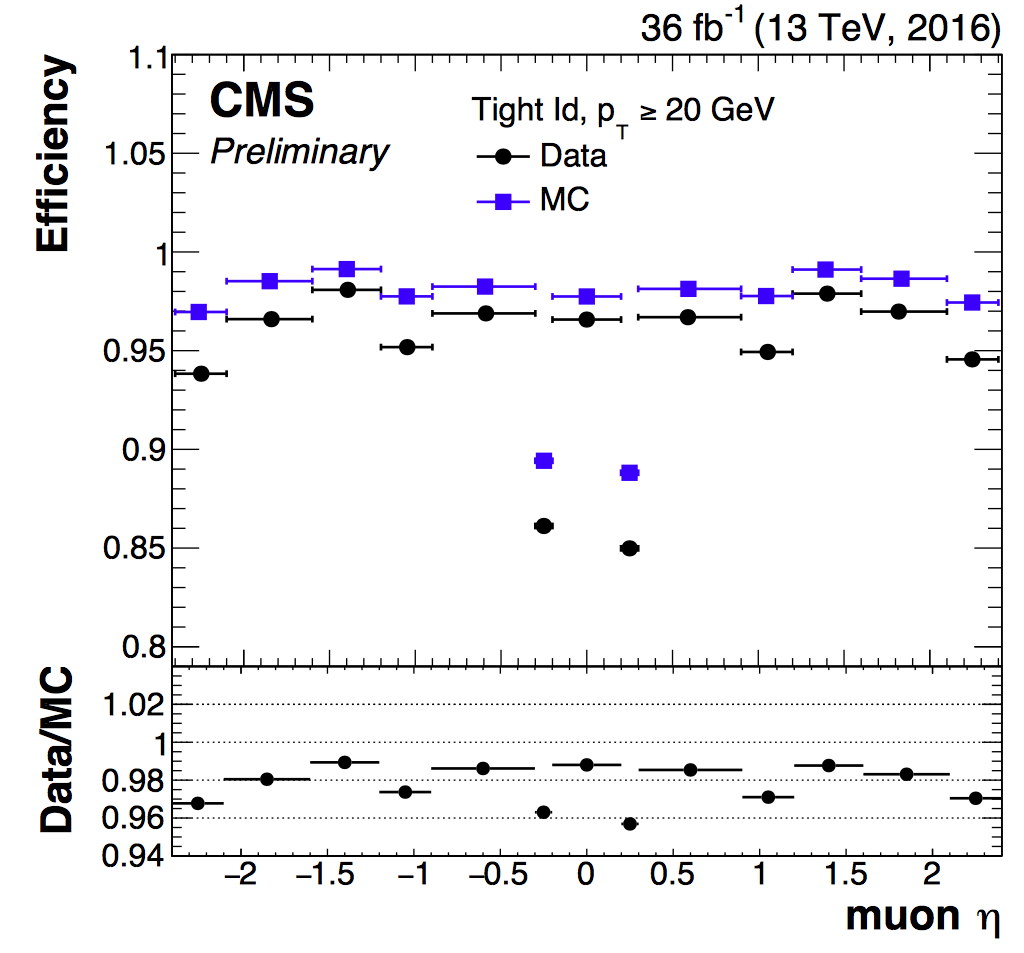
\includegraphics[width=0.495\linewidth]{4_EventRecoSelect/Figures/TightIDvseta}
	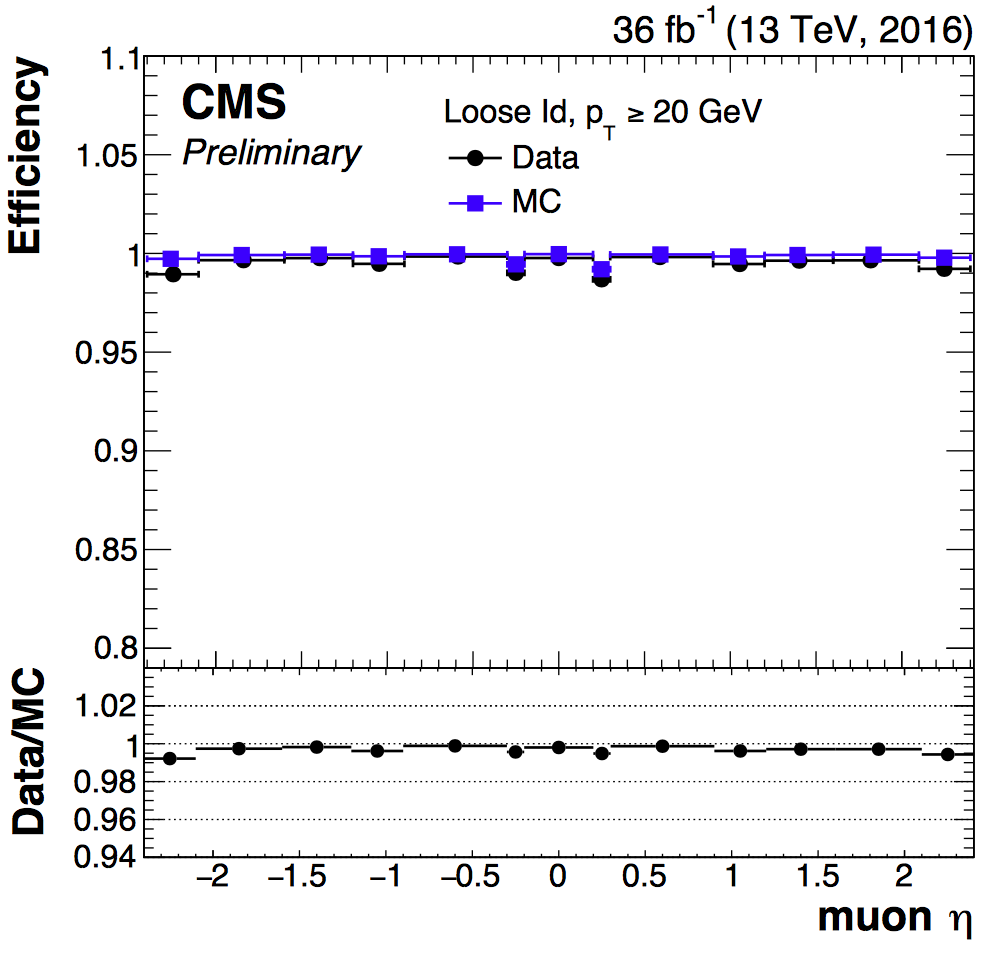
\includegraphics[width=0.495\linewidth]{4_EventRecoSelect/Figures/LooseIDvseta}
	\caption{Comparison of the muon tight ID (left) and loose ID (right) efficiencies in data and simulation as a function of the pseudorapidity of the muon using the full 2016 dataset. Figure taken from \cite{CMS-DP-2017-007}.}
	\label{fig:tightid}
\end{figure}

In addition to the identification criteria, the muons are required to be spatially isolated from electromagnetic and hadronic activity.  The relative lepton isolation is defined as estimating the total transverse energy of the particles emitted around the  direction of the lepton by defining a cone of radius $\Delta R$ in the $\eta\phi$ plane around the lepton direction. Then a summed energy is calculated from the charged hadrons (CH), neutral hadrons (NH), and photons (\Pphoton), excluding the lepton itself. This sum is then corrected to remove the energy coming from pileup interactions. The relative isolation for muons $\iso_{\Pmu}$ is defined as~\cite{CMS-PRF-14-001}:
\begin{equation}
 \iso_{\Pmu} = \frac{\sum \pt(\mathrm{CH}) + \mathrm{max}\left(0., \sum \Et(\mathrm{NH}), \sum \Et(\Pphoton) - 0.5 \times \sum \Et (\mathrm{CH})\right)}{\pt(\Pmu)},
\end{equation}
where a cone of $\Delta R = 0.4$ is adopted and the pileup mitigation is based on the  \dbeta\ correction. The \dbeta\ correction estimates the pileup energy as half of the contribution coming from charged hadrons. For tight ID muons, this relative isolation should be $\iso_{\Pmu} <0.15$, while for loose muons this should be $\iso_{\Pmu} <0.25$. % The chosen value for β is motivated by assuming equal production rates for the (π+,π0,π−) isospin triplet leading to a ratio of 1/2 for the production of neutral pions over charged ones. 
In \fig{fig:muoniso}, the isolation efficiencies as a function of the pseudo rapidities using the tag and probe method are shown for the tight muon working point. The efficiencies are 85-100\%  and have a decline for low-\pt\ muons. % These low-\pt\ muons are most likely coming from hadronic or heavy flavour decays. 
The differences between data and simulation are accounted for by applying $\eta$- and $\pt$-dependent scale factors on the simulation. 
\begin{figure}[htbp]
	\centering
	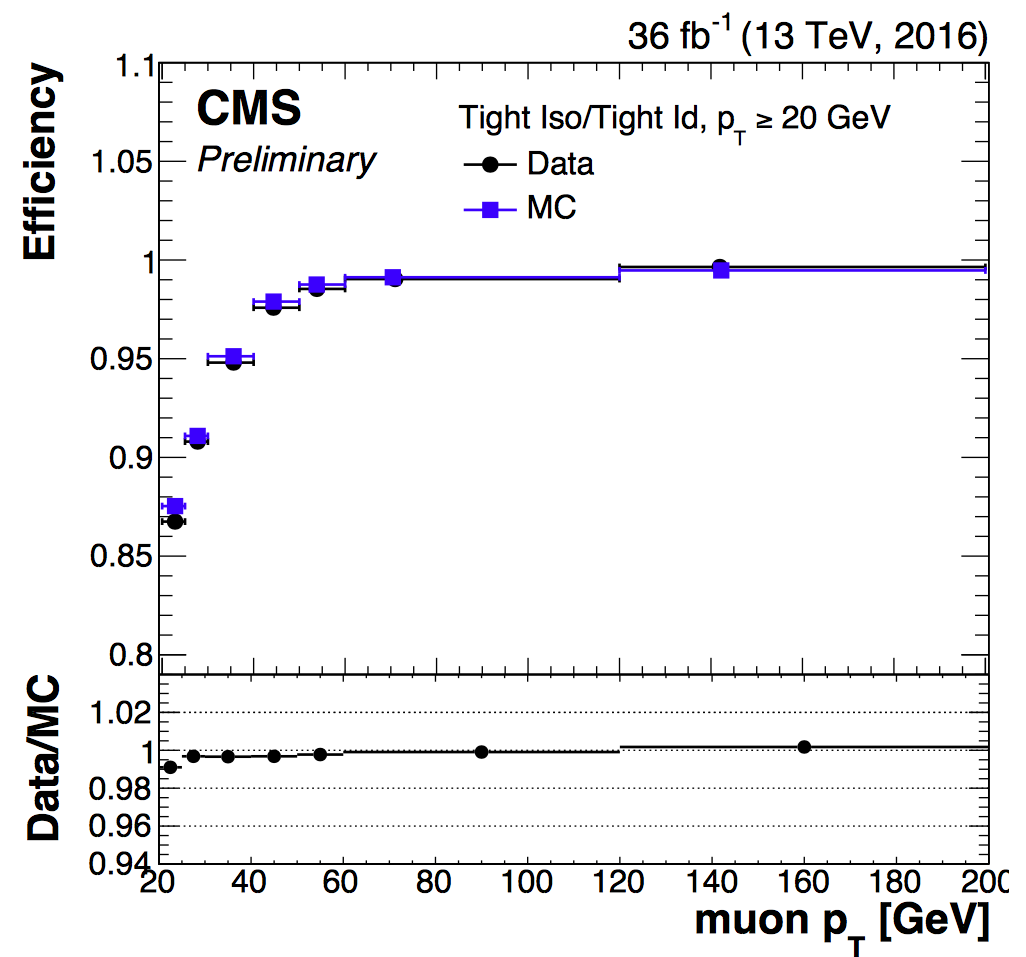
\includegraphics[width=0.494\linewidth]{4_EventRecoSelect/Figures/TightIsovsot}
	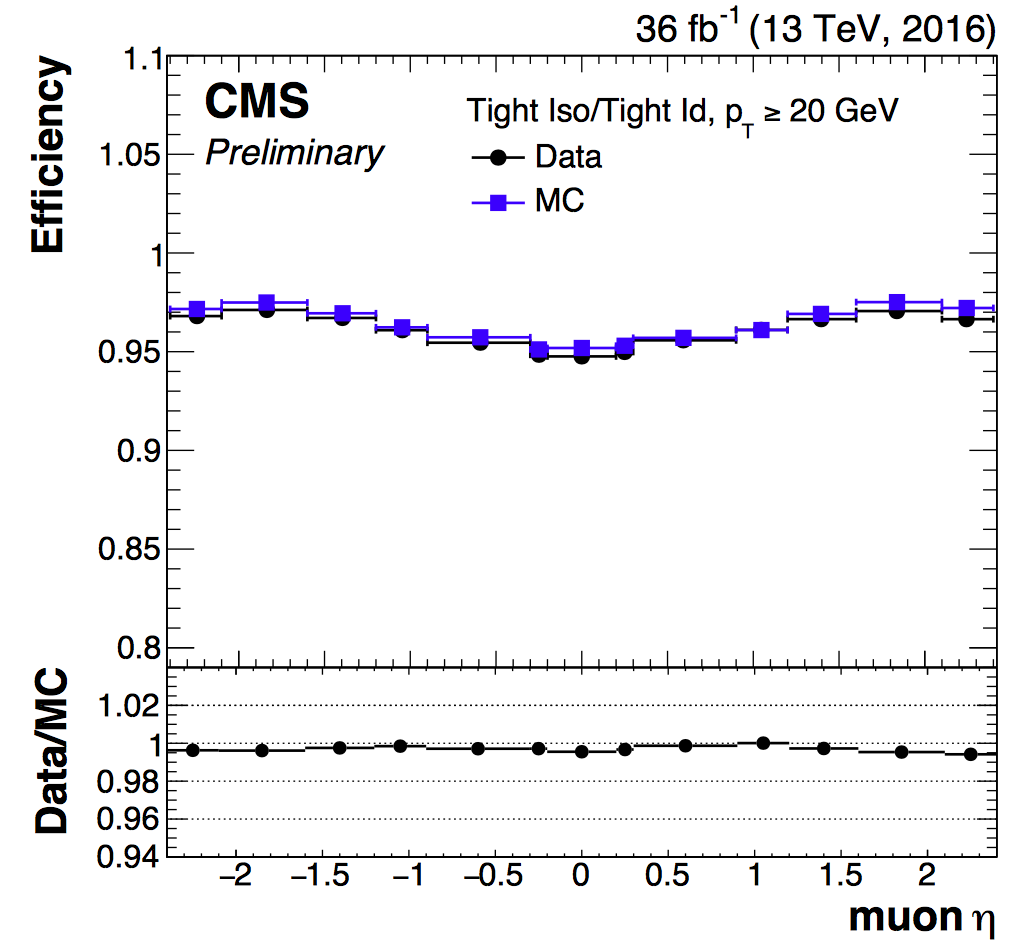
\includegraphics[width=0.494\linewidth]{4_EventRecoSelect/Figures/TightIsovseta}
	\caption{Comparison of the muon tight isolation requirement with the muon tight ID  efficiencies in data and simulation as a function of the transverse momentum (left) or  pseudorapidity (right) of the muon using the full 2016 dataset. Figure taken from \cite{CMS-DP-2017-007}.}
	\label{fig:muoniso}
\end{figure}
\begin{table}[htbp]
	\centering
	\caption{Muon requirements for the tight and loose working points, used throughout this thesis.}
	\begin{tabular}{ccc}
		\toprule
		Properties & Loose Muons & Tight Muons \\ 
		\midrule 
		Global muon or Tracker Muon & One or the other & Both \\ 
	
		Particle Flow muon & Y & Y \\ 
		
		$\chi^2/\mathrm{ndof}$ of global muon track fit & N/A & $<$ 10 \\ 
	
		Nb. of hit muon chambers & N/A & $>$ 0 \\ 
		
		Nb. of muon stations contained in the segment & N/A & $>$ 1  \\ 
		
		 Size of the transverse impact parameter  & \multirow{2}{*}{N/A }& \multirow{2}{*}{$d_{xy} < 2$ \mm} \\ 
	 of the track wrt. the PV & & \\
		Longitudinal distance wrt. the PV & N/A & $d_z < 5$ \mm \\ 
		
		Nb. of pixel hits & N/A & $>$ 0 \\ 
		
		Nb. of tracker layers with hits & N/A & $>$ 5 \\ 
	
		Relative Isolation & $<$0.25 & $<$0.15 \\
		\bottomrule
	\end{tabular} 
	
	\label{tab:MuonReq}
\end{table}


\newpage
\subsection{Electrons}
\label{sec:ElectronID}
The electron candidates used in this thesis, correspond to the tight and veto working points. The study of the electron reconstruction and identification performance can be found in \cite{CMS-DP-2017-004}.

Starting from an electron PF candidate with a GSF track that is outside the barrel-endcap transition region ($1.4443 < |\eta| <1.5660$), several requirements are set. The electron track should not have more than one (two or three) missing hit(s) in the innermost layer for the tight (veto) working point. This dismisses electrons from photon conversions. Additionally, a photon conversion veto is applied by testing if a pair of electron tracks is originating from a common displaced vertex. Furthermore, refined cuts are applied on the shower shape variables such as the difference in $\eta$ or $\phi$ between the energy weighted supercluster position in the ECAL and the track direction  at the innermost tracker position ($\Delta \eta_{\mathrm{in}}$, $\Delta \phi_{\mathrm{in}}$), and the ECAL crystal based shower covariance in the $\eta$ direction ($\sigma_{\eta \eta}$). These cuts also include energy related variables such as the absolute difference between the inverse electron energy measured in the ECAL and the inverse momentum measured in the tracker ($|1/E-1/p|$), and the ratio of the energy measured in the HCAL and ECAL (H/E). Unlike the muon case, the identification criteria also contain requirements on the isolation of the electrons.

Similar to the muons, the electron  relative isolation is determined from the sum of the particles in a cone around the electron itself. The cone radius used for electrons is $\Delta R=0.3$ and a $\rho$ correction for pileup mitigation is applied. For this correction, the expected pileup energy inside the isolation cone is estimated from the median density energy per area of pileup contamination ($\rho$), computed event by event, and the effective area ($A_{\mathrm{eff.}}$)~\cite{CMS-PRF-14-001}. This effective area is estimated from simulation and denotes the expected amount of neutral energy from pileup interactions per $\rho$ within the isolation cone as a function of the pseudorapidity of the associated ECAL superclusters. Table \ref{tab:EAeff} shows the values used for 13 \TeV\ data. The relative electron isolation $\iso_{\Pe}$  is calculated as
\begin{equation}
\iso_{\Pe} =  \frac{\sum \pt(\mathrm{CH}) + \max\left(0., \sum \Et(\mathrm{NH}), \sum \Et (\gamma) - \rho \times A_{\mathrm{eff.}}\right)}{\pt(\Pe)}.
\label{eq:drho}
\end{equation}
\begin{table}[htbp]
	\centering 
	\caption{The effective areas  $A_{\mathrm{eff.}}$ used for the electron relative isolation~\cite{ilya}.}
	\begin{tabular}{cc}
		\toprule 
		$\eta$ region  & $A_{\mathrm{eff.}}$ \\ 
		\midrule
		$0<|\eta| < 0.1752$ & 0.1703 \\ 
	
		$1.0<|\eta| < 0.1479$ & 0.1715 \\ 
	
		$1.479<|\eta| < 2.0$ & 0.1213 \\ 
	
		$2.0<|\eta| < 2.2$ & 0.1230 \\ 
	 
		$2.2<|\eta| < 2.3$ & 0.1635 \\ 
	
		$2.3<|\eta| < 2.4$ & 0.1937 \\ 
		 
		$2.4<|\eta| < 2.5$ & 0.2393 \\ 
		\bottomrule
	\end{tabular} 
	\label{tab:EAeff}
\end{table}

The efficiency of electron identification is estimated from $\PZ \rightarrow \Pelectron \APelectron$ events via the tag-and-probe method and is shown in \fig{fig:electrontightidvspt} for the tight working point. The efficiencies reach $95-100$\%.  The difference between  data and  simulation is corrected for by dedicated $\pt$- and $\eta$ dependent scale factors as well. 
\begin{figure}[htbp]
	\centering
	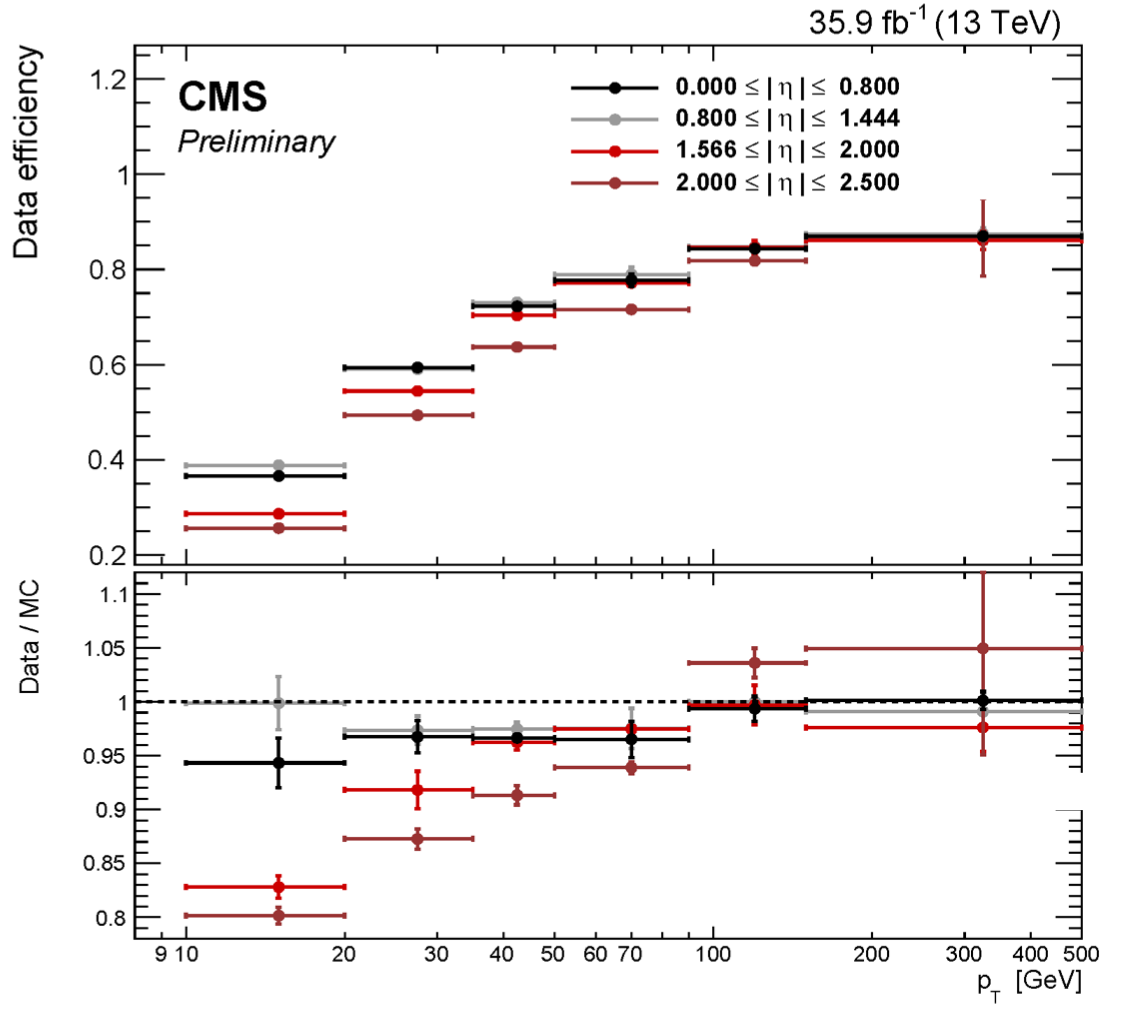
\includegraphics[width=0.7\linewidth]{4_EventRecoSelect/Figures/ElectronTightIDvsPt}
	\caption{Electron identification efficiency as function of the electron transverse momentum from the full 2016 dataset. Figure taken from \cite{CMS-DP-2017-004}.}
	\label{fig:electrontightidvspt}
\end{figure}

\begin{table}[htbp]
	\centering
	
	\caption{Electron requirements used in this analysis. The requirements are set in the barrel ($|\eta_{supercluster}| \leq 1.479$)
		and the endcaps ($|\eta_{supercluster}| > 1.479$). }
	\begin{tabular}{ccccc}
		\toprule
		Properties & \multicolumn{2}{c}{$|\eta_{supercluster}| \leq 1.479$ } & \multicolumn{2}{c}{$|\eta_{supercluster}| > 1.479$ } \\
		
		& Veto electron & Tight electron & Veto electron & Tight electron \\ 
	  \midrule
		$ \sigma_{\eta \eta}$ & $<$ 0.0115 & $<$ 0.00998 & $<$ 0.037 & $<$ 0.0292 \\ 
	
		$|\Delta \eta_{\mathrm{in}}|$ & $<$ 0.00749 & $<$ 0.00308 & $<$ 0.00895& $<$ 0.00605\\ 
	 
		$|\Delta \phi_{\mathrm{in}}|$ & $<$ 0.228 & $<$ 0.0816 & $<$ 0.213& $<$ 0.0394 \\ 
		
		H/E & $<$ 0.356 & $<$ 0.0414 & $<$ 0.211& $<$ 0.0641 \\ 
		
		relative isolation & $<$ 0.175 & $<$ 0.0588  & $<$ 0.159& $<$ 0.0571\\ 
	
		$|1/E-1/p|$ (\GeVinv) & $<$ 0.299 & $<$ 0.0129 & $<$ 0.15 &$<$ 0.0129 \\ 
	
		expected missing inner hits & $\leq $ 2 & $\leq $ 1 &  $\leq $ 3 &  $\leq $ 1\\ 
		%		\hline
		%		d0 - dz & 0.05 cm & 0.05 cm & 0.10 cm & 0.10 cm \\
		
		 conversion veto & Y & Y & Y & Y\\ 
		\bottomrule
	\end{tabular} 
	\label{tab:ElecReq}
\end{table}


\subsection{Jets}
\label{sec:JetID}
%https://twiki.cern.ch/twiki/bin/view/CMS/IntroToJEC
Jets are reconstructed  from all reconstructed particles without the charged hadrons associated to pileup vertices. The clustering is done with the \antikt\ algorithm~\cite{Cacciari:2008gp} with a radius parameter for the cone size of the resulting jet of $R=0.4$. %The initial step of the \antikt\ algorithm considers all candidates as ''protojets" and starts to calculate the distances for protojets i and j as
%\begin{equation}
%\begin{aligned}
%   d_{\mathrm{ij}} &= \mathrm{min}\left(\frac{1}{p_{\mathrm{T,i}}^2}, \frac{1}{p_{\mathrm{T,j}}^2}\right), \\
%   d_{\mathrm{i}} &= \frac{1}{p_{\mathrm{T,i}}^2}.
% \end{aligned}
%\end{equation}
%For each iteration the two distances are calculated. When $d_{\mathrm{ij}} < d_{\mathrm{i}}$, the two protojets are merged and their four momentum is summed. If $d_{\mathrm{i}}$ is the smallest distance, the protojet is renamed as final jet and ignored in the subsequent steps. 
More information about the jet algorithm performance can be found in Ref. \cite{CMS-PAS-JME-16-003}.

The jets used for the analysis  in this thesis, are identified according to the loose identification working point summarised in \tab{tab:jetID}. The requirements on the jet constituents are based on the assumption that a proper jet originating from the hadronisation of a quark or gluon consists of multiple PF particles and types. Therefore, the jet should consists of more than one constituent, and the neutral hadron fraction and neutral EM energy fractions should be less than 99\%. For the jets within the tracker acceptance ($|\eta|<2.4$), at least one constituent has to be a charged hadron resulting in a charged hadron energy fraction above 0\%. Additionally the charged EM energy fraction should be less than 99\%. On top of these requirements, objects that are labelled as jets and found in the vicinity of any isolated lepton, $\Delta R < 0.3$, are removed from the jet collection in that event to avoid duplications of objects. 
\begin{table}[h]
	\centering
	\caption{Jet criteria used throughout the thesis. The last three requirements are only for jets within the tracker acceptance.}
	\begin{tabular}{cc}
		\toprule 
		Properties & Loose Jet ID \\ 
		\midrule
		Neutral hadron fraction & $<$ 0.99 \\ 
		
		Neutral EM fraction & $<$ 0.99 \\ 
		
		Number of constituents & $>$ 1 \\ 
		 		
		Charged hadron fraction & $>$ 0 \\ 
	 
		Charged multiplicity & $>$ 0 \\ 
		
		Charged EM fraction & $<$ 0.99 \\ 
		\bottomrule
	\end{tabular} 
	\label{tab:jetID}
\end{table}

The energy of the reconstructed jets deviates from the energies of the corresponding jets clustered from the hadronisation products of true partons from simulations due to non-linear subdetetector responses and efficiencies. The jet energy corrections (JEC) calibrate the jets in order to have the correct energy scale and resolution.
Jet energy scale corrections (JES) are determined as a function of pseudorapidity and the transverse momentum from data and simulated events by combining several channels and methods. This is extensively described in Ref.~\cite{1748-0221-12-02-P02014}. These corrections account for the effects of pileup, the uniformity of the detector response, and residual data-simulation jet energy scale differences. Furthermore, the jet energy resolution (JER) is measured in data and simulation as a function of pileup, jet size and jet flavour.  %A detailed understanding of both the energy scale and the transverse momentum resolution of the jets is crucial for many physics analysis, and these are commonly the main source of systematic uncertainty.
 The performance of the jet energy corrections for the 13 \TeV\ dataset can be found in Ref. \cite{CMS-DP-2016-020}.


The JEC are factorised and subsequently correct for the off-set energy due to pileup, the detector response to hadrons, and residual differences between data and simulation as a function of the jet pseudorapidity and transverse momentum.  The consecutive steps of JEC are shown in \fig{fig:jes}. 
\begin{figure}[htbp]
	\centering
	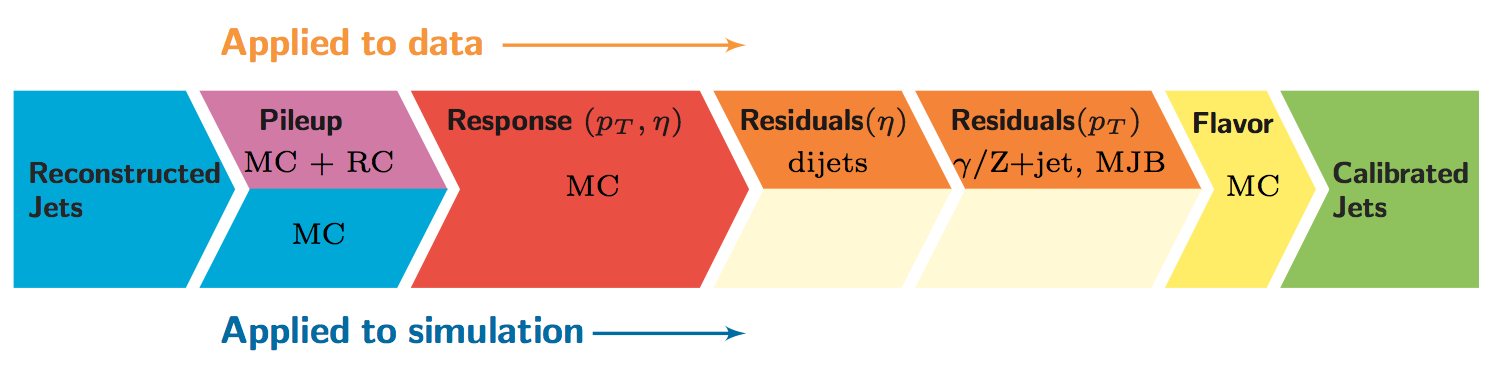
\includegraphics[width=1.\linewidth]{4_EventRecoSelect/Figures/JES}
	\caption{The sequence of the JEC for data and simulations The corrections marked with MC are derived from simulation studies, while RC stands for random cone, and MJB for the analysis of multi-jet events. Figure taken from \cite{1748-0221-12-02-P02014}.}
	\label{fig:jes}
\end{figure}
The off-set corrections remove the dependency of the jet energy response of additional pileup activity. It is based on the jet area method, which uses the effective area of the jets multiplied by the average density in the event, to calculate the off-set energy to be subtracted from the jets.  The correction factors are derived by comparing the jet response with and without pileup events. The residual differences between data and detector simulation are determined using the random cone method (RC). For this method, many jets are reconstructed in each event by clustering particles through placing  random cones. This provides a mapping of the $\eta\phi$ plane and the average \pt\ of those jets gives the average energy off-set due to pileup~\cite{1748-0221-12-02-P02014}. 
The next level of corrections have as goal to have a uniform energy response independent of the transverse momentum or pseudorapidity of the jet.  These corrections are determined from simulated events by matching the reconstructed jets to true particle jets and comparing their momenta. 
The residual corrections between data and simulation are determined by comparing the transverse momentum balance in various types of events (multi-jet, \Zjets, and \pjets), using a reference jet in the barrel region.  
The jet flavour corrections are optional and not used for this thesis. More information on the jet flavour corrections can be found in Ref.~\cite{1748-0221-12-02-P02014}. For jets with a transverse momentum above 30~\GeV, the uncertainties from the various corrections are 3-5\% for the 13~\TeV\ dataset~\cite{CMS-DP-2016-020}.


After applying JEC, the transverse momentum resolution of the jet is extracted from data and simulated events. There are two methods used to rescale the reconstructed four momentum based on whether or not the simulated jet can be matched to a true jet  in simulation. The factors are defined as
\begin{equation}
\begin{aligned}
c_{\mathrm{matched}} &= 1 + \frac{\pt^{\mathrm{reco.}}-\pt^{\mathrm{true}}}{\pt^{\mathrm{reco.}}} \left(s_{\mathrm{JER}} -1\right), \\
c_{\mathrm{unmatched}} &= 1 + \mathrm{N}(0, \sigma_{\mathrm{JER}})\sqrt{\mathrm{max}\left(s^2_{\mathrm{JER}}-1, 0\right)},
\end{aligned}
\end{equation}
where $ \mathrm{N}(0, \sigma_{\mathrm{JER}})$ denotes a sample value from a normal distribution centred at zero with as standard deviation the relative resolution in simulation $\sigma_{\mathrm{JER}}$, and $s_{\mathrm{JER}}$ the $\eta$-dependent resolution scale factors. These scale factors are derived in data from di-jet or \pjets\ events and analysing the \pt\ balance. The resolution scale factors (data/simulation) are found to be 1.1-1.2~\cite{CMS-DP-2016-020}. %, except for the EC-HF transition regions around $|\eta| =3$ and $|\eta| = 1.4$~\cite{CMS-DP-2016-020}.

%\begin{figure}[htbp]
%	\centering
%	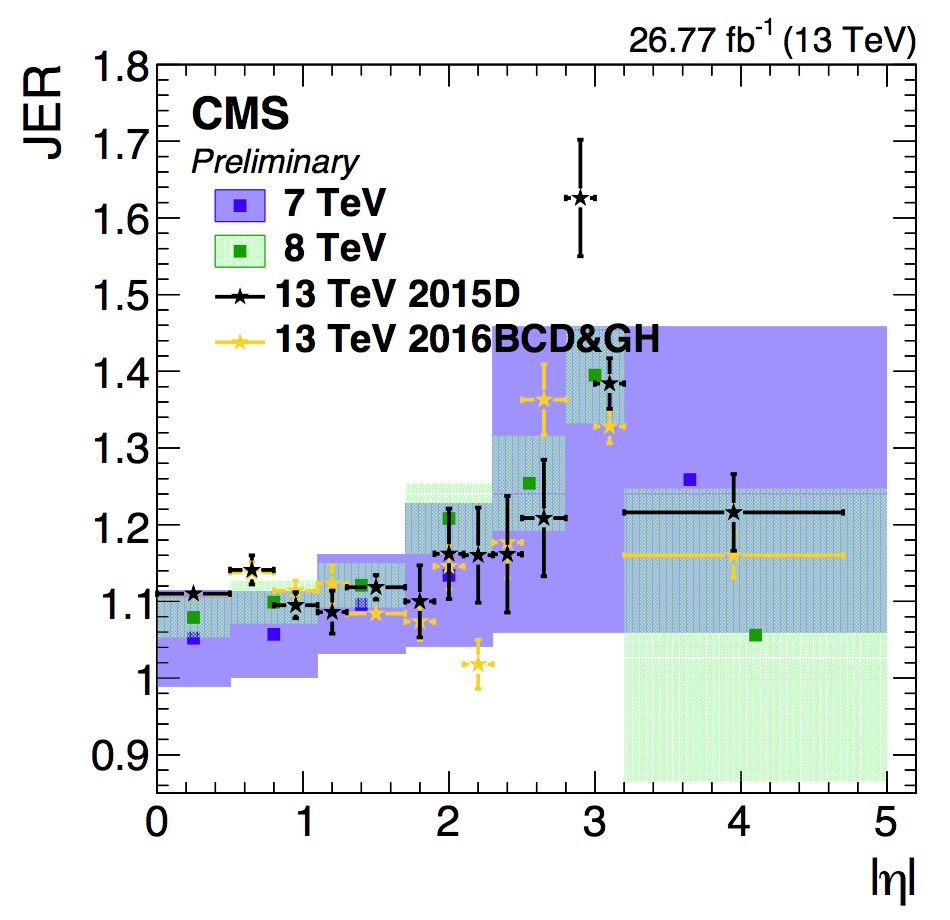
\includegraphics[width=0.7\linewidth]{4_EventRecoSelect/Figures/JERSF}
%	\caption{Data/MC scale factors for the jet energy resolution evaluated on di-jet events. Figure taken from~\cite{CMS-DP-2016-020}.}
%	%https://indico.cern.ch/event/595771/contributions/2412097/attachments/1391113/2119307/20161220_Marek_2016_combined_result_w_wo_FwdExtention.pdf
%	\label{fig:JER}
%\end{figure}

%\begin{table}[htbp]
%	\centering
%	\caption{Jet energy resolution factors in bins of $\eta$ with uncertainty}
%	\begin{tabular}{ccc}
%		\toprule
%		$|\eta|$ & SF & Uncertainty ($\pm$) \\ 
%		\midrule
%		0-0.5 & 1.109 & 0.008 \\ 
%
%		0.5-0.8 & 1.138 & 0.013 \\ 
%
%		0.8-1.1 & 1.114 & 0.013 \\ 
%
%		1.1-1.3 & 1.123 & 0.024 \\ 
%	
%		1.3-1.7 & 1.084 & 0.011 \\ 
%	
%		1.7-1.9 & 1.082 & 0.035 \\ 
%	
%		1.9-2.1 & 1.140 & 0.047 \\ 
%	
%		2.1-2.3 & 1.067 & 0.053 \\ 
%	
%		2.3-2.5 & 1.177 & 0.041 \\ 
%		\bottomrule
%	\end{tabular} 
%	\label{tab:JER}
%\end{table}

\subsection{Jets from b quark fragmentation}
\label{sec:BJetID}
Jets originating from the hadronisation of bottom quarks can be discriminated from jets from gluons and light-flavour quarks as well as charm quark fragmentation through the use of b-tagging. There are several algorithms developed within CMS to perform b-tagging~\cite{1748-0221-8-04-P04013,CMS-PAS-BTV-15-001} on jets that fall within the pseudorapidity acceptance of the trackers. These algorithms exploit the properties of the \Pbottom\ quark to identify the jets formed by its fragmentation. These hadrons have relative large masses, long lifetimes and daughter particles with hard momentum spectra. Additionally, their semi-leptonic decays can be exploited as well.  To use b jet identification in an analysis, one needs to know its efficiency and misidentification probability. In general, these are function of the pseudorapidity and transverse momentum of the considered jet. Their performances are directly measured from data by use of b jet enriched jet samples (multi-jet or top-quark decays). 


This thesis uses b jets identified by the Combined Secondary Vertex version 2 (CSVv2) algorithm~\cite{1748-0221-8-04-P04013}. This algorithm combines secondary vertices together with track based lifetime information by use of a multivariate technique. The secondary vertex is reconstructed from displaced tracks within a jet, as illustrated in \fig{fig:btaggingdiagram}. The final state b quark provides a B meson (e.g. B$^{\pm}$, B$_0$, B$_{\mathrm{S}}$) after the hadronisation. This B meson has a relatively long lifetime and can travel a measurable distance from the primary vertex before decaying. %\footnote{For example, B$^{\pm}$ mesons have a lifetime of about 1.6 ps~\cite{PDG} and travel 4-9 mm before decaying if their momenta is 40-100 \GeV.}.
 After reconstruction, the secondary vertices are required to be in accordance with the B meson hypothesis based on the amount of shared tracks with the primary vertex, the invariant vertex mass to reject kaon decays, and the direction of the tracks compared to the jet axis. 
\begin{figure}[htbp]
	\centering
	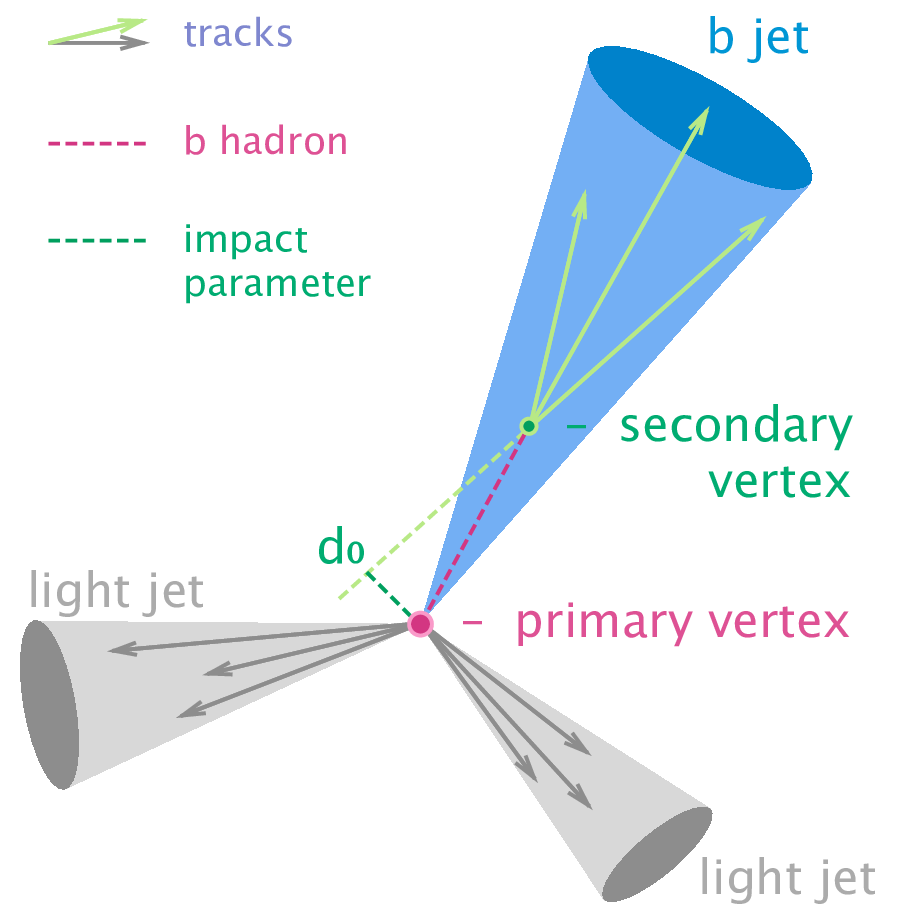
\includegraphics[width=.5\linewidth]{4_EventRecoSelect/Figures/B-tagging_diagram}
	\caption{Sketch showing the common principle of the identification of b jets. Figure taken from \cite{btagjet}.}
	\label{fig:btaggingdiagram}
\end{figure}

The b-tagging algorithm performances are evaluated taking into account two cases: discrimination of b-tagged jets originating from charm quarks, and discrimination of b-tagged jets against jets coming from gluons or light (\Pup, \Pdown, \Pstrange) quarks. In \fig{fig:figure008}, the misidentification probabilities for different b-tagging algorithms within CMS are shown.
Different working points  are defined based on the misidentification probabilities for a certain threshold on the CSVv2 discriminator. These are shown in \tab{tab:bctag}. The analysis presented in this thesis uses the loose working point which has an average efficiency of 81\% and a misidentification probability of 10\%. \todo{Find reason why I am not using cMVA, omdat CVSv2 op ttbar events is gemeten en cMVA op multijet?  cMVA scalefactors zijn enkel bepaald voor ttbar onde r200 gev omdat hiervoor ook leptoninfo wordt gebruikt in het algoritme en er is bias als je SF bepaald met dezelfde lepton info, Deep CSV met NN is er nu ook met betere improvement tov CSVv2, deep flavour }
\begin{figure}[htbp]
	\centering
	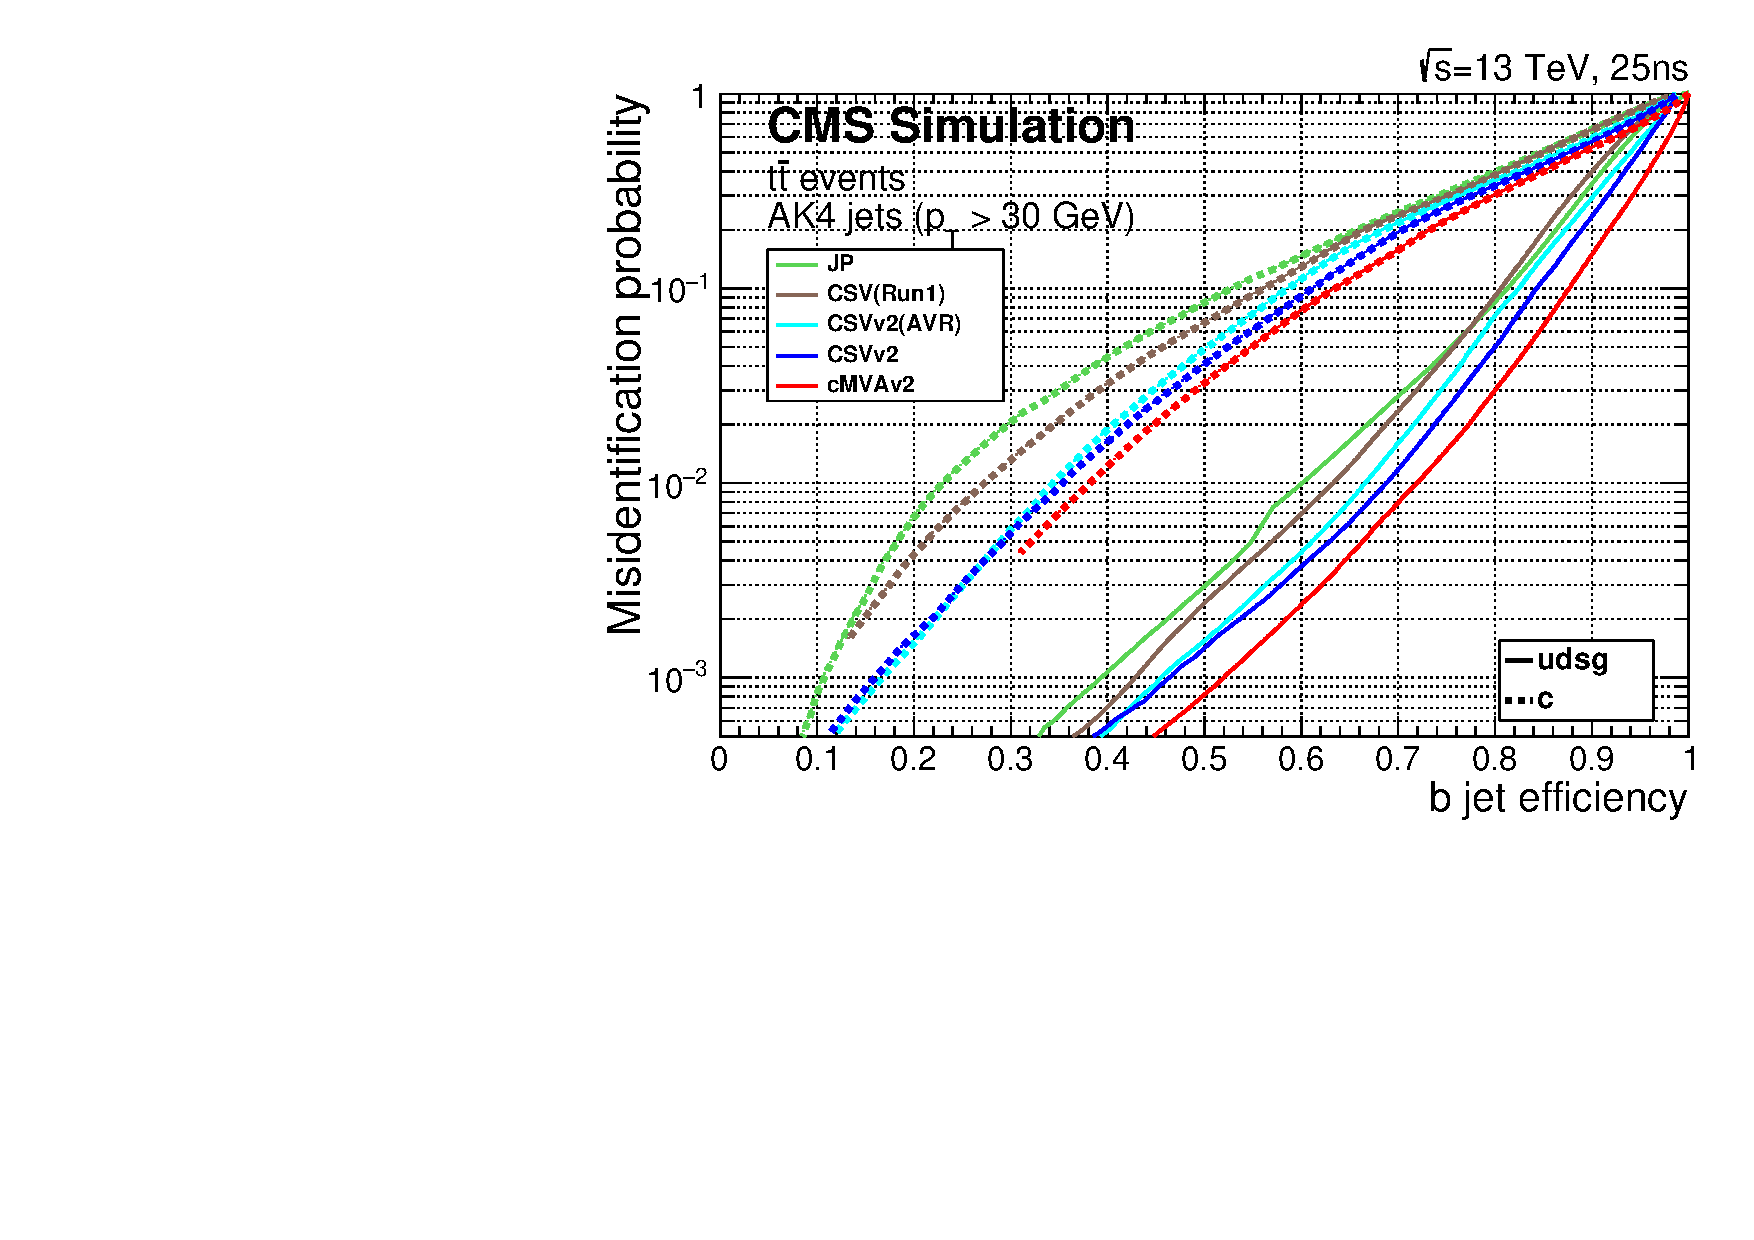
\includegraphics[width=0.7\linewidth]{4_EventRecoSelect/Figures/Figure_008}
	\caption{Misidentification probabilities of various b-tagging algorithms in simulation. Figure taken from \cite{CMS-PAS-BTV-15-001}. }
	\label{fig:figure008}
\end{figure}
\begin{table}[htbp]
	\centering
	\caption{Working points used for tagging jets as coming from b quarks for the CSVv2 discriminant.}
	\begin{tabular}{cccc}
		\toprule
		WP  & CSVv2 discr cut & b-tag eff. & misid. prob. \\ 
		\midrule
		Loose (L) & $>$ 0.5426 & $\approx 81\%$ &  $\approx 10\%$ \\ 
	
		Medium (M)& $>$ 0.8484 & $\approx 66\%$ &  $\approx 1\%$\\ 
		
		Tight (T) & $>$ 0.9535 & $\approx 46\%$ &  $\approx 0.1\%$\\ 
		\bottomrule
	\end{tabular} 
% see http://cms.cern.ch/iCMS/analysisadmin/cadilines?line=BTV-16-002
	\label{tab:bctag}	
\end{table}
\newpage
The efficiency of tagging a jet as coming from a bottom quark in simulation typically deviates somewhat from data. Efficiency scale factors $\epsilon^{\mathrm{data}}_{\Pbottom}/\epsilon^{\mathrm{MC}}_{\Pbottom}$ are derived from data to account for those differences. These scale factors are $\eta$-, $\pt$-, and flavour-dependent, where the flavour of the jet is determined from matched generated hadrons. For cut based analyses these scale factors are applied to the b-tagging efficiencies and mistag probabilities according to the chosen working point~\cite{CMS-PAS-BTV-15-001}. For shape-based analyses however, such as the one presented in this thesis, the scale factors are applied on the distribution of the b-tagging discriminator. This is the so-called IterativeFit method~\cite{CMS-PAS-BTV-16-001}. %It uses a tag and probe method to measure the scale factors for both b, c, and  light flavoured jets simultaneously. The scale factors to account for the differences in simulation and data for the probe jet are determined iteratively to account for the impact of the b-, c-flavour, and light flavour scale factors on eachother. In a fist step, no scale factors are applied. Then the scale factor is measured by applying the scale factors of the previous iteration to simulation until the scale factors become stable. Throughout the procedure, the scale factor for charm jets are set unity with an uncertainty that is twice the one of the b scale factor. The scale factors obtained in $\eta$-, \pt-, and CSVv2 discriminant values are determined with the bin content N of the considered ($\eta$,\pt,discriminant) bin as
%\begin{equation}
%\begin{aligned}
%\mathrm{SF}_{\Pbottom} &= \frac{N_{\Pbottom}^{\mathrm{data}} - N_{\Pbottom}^{\mathrm{MC}}}{N_{\Pbottom}^{\mathrm{MC}}}, \\
%\mathrm{SF}_{\Pgluon, \Pup,\Pdown, \Pstrange} &= \frac{N_{\Pgluon, \Pup,\Pdown, \Pstrange}^{\mathrm{data}} - N_{\Pgluon, \Pup,\Pdown, \Pstrange}^{\mathrm{MC}}}{N_{\Pgluon, \Pup,\Pdown, \Pstrange}^{\mathrm{MC}}}, \\
%\mathrm{SF}_{\Pcharm} &= 1. 
%\end{aligned}
%\end{equation}

 The uncertainties related to the IterativeFit method cover the possible shape discrepancies between data and simulation. There are two uncertainties coming from the purity of the sample based on the purity of the light flavoured (lf) and heavy flavoured (hf) jet contributions in the sample. Furthermore, the jet energy scale results in jets migrating from one \pt\ bin to another and has an influence on the bin dependent scale factors. Also the statistical fluctuations of the limited amount of entries in each bin are accounted for and have an influence on the scale factor uncertainties. The statistical fluctuations  have four uncorrelated sources: two for heavy flavour and two for light flavour jets.  The uncertainty on the scale factors for the jets originating from a charm quark (cf) is determined from the uncertainty on the scale factors from a bottom quark, and results in two independent uncertainties~\cite{CMS-PAS-BTV-16-001}.


\subsection{Missing transverse energy}
\label{sec:MET}
The missing transverse momentum \ptmisvec\ and energy \Etmis\ resulting from particles that do not interact with the detector material, are calculated by balancing the vectorial sum of the transverse momenta of all particles: 
\begin{equation}
\begin{aligned}
	\Et &= \left|\ptmisvec\right|, \\
	\ptmisvec &= - \sum \limits_{\mathrm{i} = 1}^{\mathrm{N}_{\mathrm{particles}}} \vec{p}_{\mathrm{T,i}}.
\end{aligned}	
\end{equation}
%The $z$-component can not be calculated from the momentum imbalance since the boost along the $z$-axis, determined by the momentum fraction, can not be reconstructed. 

The missing transverse energy is influenced by the minimum thresholds in calorimeters, the inefficiencies in the tracker, and the non-linear response of the calorimeter to hadronic particles. The bias is reduced by correcting the transverse momentum of the jets to particle jet \pt\ via the JEC and propagating it to the  missing transverse momentum.
%\begin{equation}
%\begin{aligned}
%\ptmisvec^{\mathrm{corr}} &= - \sum \limits_{\mathrm{i} = 1}^{\mathrm{N}_{\mathrm{jets}}} \vec{p}_{\mathrm{T,i}}^{\mathrm{corr.}}  - \sum \limits_{\mathrm{i} = 1}^{\mathrm{N}_{\mathrm{unclustered}}} \vec{p}_{\mathrm{T,i}}^{\mathrm{raw}}, \\
%\ptmisvec^{\mathrm{corr}} &= \ptmisvec^{\mathrm{raw}} - \sum \limits_{\mathrm{i} = 1}^{\mathrm{N}_{\mathrm{jets}}} \left( \vec{p}_{\mathrm{T,i}}^{\mathrm{JEC}}  - \vec{p}_{\mathrm{T,i}}^{\mathrm{PU-only}}\right). 
%\end{aligned}
%\end{equation}
%The $ \vec{p}_{\mathrm{T,i}}^{\mathrm{PU-only}}$ denotes the transverse momentum of the jet, where only the pileup related corrections are applied. 
The performance of the missing transverse energy reconstruction can be found in \cite{CMS-PAS-JME-16-004}. 
\newpage
\section{Summary of corrections}
\label{sec:SummaryCor}
Throughout the chapter several corrections are introduced to improve the agreement between data and simulation. These corrections are sources of systematic uncertainties for the analysis presented in this thesis. Therefore a summary of the corrections and their associated uncertainties is provided. 
% HIP EFFECT https://indico.cern.ch/event/560224/contributions/2265347/attachments/1320462/1980048/WGM_HIP_Boudoul.pdf
%https://hypernews.cern.ch/HyperNews/CMS/get/recoTracking/1726/1/1/1.html
\begin{description}
  		\item[Lepton scale factors] The systematic uncertainty on the lepton scale factors consists of three sources: identification, isolation and tracking.	The applied scale factors are varied independently within one standard deviation of their measured uncertainties to account for their systematic impact on the measurements. 

	\item[Jet energy corrections] The momenta of the reconstructed jets are corrected to match on average the expected true energy derived from the hadronisation products of partons in simulation. Furthermore, residual corrections and smearing is applied to match the overall energy scale and resolution for simulation and data. These corrections are also propagated to the missing transverse energy. The systematic uncertainties due to these scale factors are estimated by varying them within their uncertainties and repeating the measurements with recalibrated jets and missing transverse energy. 
	

	
	\item[CSVv2 discriminant shape reweighting] There are three sources of uncertainty contributing to the measurement of the scale factors: statistical uncertainties, jet energy scale and the purity of the sample. The jet energy scale uncertainty is 100\% correlated to the jet energy uncertainties and is evaluated simultaneously. The uncertainty coming from the purity of the sample is subdivided into two uncorrelated uncertainties based on the purity of the light flavoured (lf) and heavy flavoured (hf) jet contributions in the sample. A one sigma shift in each of the two purity contributions corresponds to a higher/lower contribution in the purity of the considered flavours. The statistical uncertainties have four uncorrelated sources, two for heavy flavour and two for light flavour jets. One of the uncertainties correspond to the shift consistent with the statistical uncertainties of the sample, while the other is propagated in a way that the upper and lower ends of the distribution are affected with respect to the centre of the distribution.   The uncertainty on the charm jet scale factors (cf)   is obtained from the uncertainty on the heavy flavour scale factors, doubling it in size and constructing two nuisance parameters to control the charm flavour scale factors and treating them as independent uncertainties. 
	
	
		\item[Pileup] Varying the minimum bias cross section, used to calculate the pileup distribution by $\pm$4.6\%, results in a systematic shift in the pileup distribution. The uncertainty is estimated by recalculating the pileup weights to the distributions associated to the minimum bias cross sections. 
		
		
		\item[Luminosity] The luminosity  is measured with a global uncertainty of 2.5\%, affecting the expected number of events. 
	
\end{description}

\begin{comment}
% Jet energy scale and resolution in the CMS experiment in pp collisions at 8 TeV
% http://iopscience.iop.org/article/10.1088/1748-0221/12/02/P02014/meta
% atlas http://inspirehep.net/record/1519834

% photobn http://iopscience.iop.org/article/10.1088/1748-0221/10/08/P08010/pdf
\subsection{The particle flow event reconstruction method}
% https://cds.cern.ch/record/2237475?ln=en
% atlas http://inspirehep.net/record/1520722
\subsection{Identification of particles}
\subsubsection{Muon reco and ID}
% trigger and good explenation of ID https://arxiv.org/pdf/1206.4071.pdf
% https://cds.cern.ch/record/2257968/files/DP2017_007.pdf
\subsubsection{Electron reco and ID}
% https://cds.cern.ch/record/2255497/files/DP2017_004.pdf
% https://cds.cern.ch/record/2255497?ln=en
\subsubsection{Jet reco and ID of b quarks}
% jet algorithms 
% http://cms.cern.ch/iCMS/analysisadmin/cadi?ancode=JME-16-003

% Identification of b and c jets in the CMS experiment at the LHC Run 2
% http://cms.cern.ch/iCMS/analysisadmin/cadilines?line=BTV-16-002
% SF https://twiki.cern.ch/twiki/bin/view/CMS/BtagRecommendation80XReReco
%Identification of b quark jets at the CMS Experiment in the LHC Run 2
% https://cds.cern.ch/record/2138504?ln=en

%Identification of c-quark jets at the CMS experiment
%https://cds.cern.ch/record/2205149?ln=en

\subsubsection{Missing transverse energy reconstruction}
\subsection{Calibrations and corrections}
%CMS has been taking collision data since the 13TeV startup of the LHC on 3 June. During this period, the CMS magnet has been kept off due to an issue with the cooling system, so the beams have been used to calibrate and time-in the electronics of the various parts of the detector. These operations, which are largely independent of the magnetic field, are now complete. Meanwhile, the data collected with zero magnetic field can be used for fundamental research, like the measurement of the multiplicity of charged particles produced at the new collision energy of 13 TeV. The issue with the magnet cooling system was identified in the final preparatory phase leading to collisions in the LHC. While preparing for beam in CMS, a problem was found in the system that feeds liquid helium to the CMS superconducting magnet. The problem was diagnosed to be due to oil, which is used in the initial compression stages, reaching the so-called 'cold-box’ of the cryogenic system. The cold-box is a complex system with several sets of filters protecting three turbines along the path of the helium towards the magnet. In order to clean the oil contamination essentially all components of the cold-box have been extracted and replaced. Analysis confirms that there is no oil contamination in the CMS magnet itself or risk to its operation during 2015. The cold-box of is now being stabilised after the cleaning intervention and is being brought back to operational conditions. CMS is confident that, following the LHC technical stop and the beam conditioning run that will start at the end of this week, after the low-intensity and commissioning period, the full magnetic field will be available for the 13 TeV LHC run.
\end{comment}






